% =====================================================================
%  CHAPTER 5 — DATASET AND EVALUATION
%  Zero-Shot Nutrient and Quantity Association using
%  OCR-Guided Semantic Graph Matching
%  Moustafa Hamada | THD + USB
%
%  Build: scrbook, XeLaTeX + BibTeX. Citations: \cite{}. Cross-refs: \S\ref{}.
%  Packages used here (graphicx, booktabs, placeins) are already loaded
%  for Chapter 4 -- nothing new to add to the preamble.
%
%  LABELS USED IN THIS FILE (align to your actual labels if they differ):
%    chap:evaluation
%    sec:corpus, sec:schema (+ -tuple, -annotation, -normalisation),
%    sec:fields (+ -nutrient, -quantity, -unit, -context)
%    chap:methodology (Ch4), chap:experiments (Ch6)
%    fig:tuples-per-image, fig:nutrient-top15, fig:unit-distribution,
%    fig:context-structure, tab:density-bands, tab:schema, tab:quantity-formats
%
%  FIGURE ASSETS (place next to thesis.tex, as for the Ch4 figures; each is
%  guarded by \IfFileExists so the chapter compiles before they are present):
%    tuples_per_image_hist.png, nutrient_top15.png,
%    unit_distribution.png, context_structure.png
% =====================================================================

\chapter{Dataset and Evaluation}\label{chap:evaluation}

This chapter describes the data used to evaluate the pipeline of
Chapter~\ref{chap:methodology}, and how the pipeline is scored. It has two
parts. The first part describes the corpus: its size, the content of each
field, and its layout. The second part defines the evaluation metric and
the tuple-matching rules used in Chapter~\ref{chap:experiments}.

\section{Corpus Overview}\label{sec:corpus}

The corpus has $57$ images of nutrition labels from food and supplement
products. Some were provided by the thesis supervisor; the rest are
photographs of similar labels taken by the author in shops. Each image was
annotated as a set of tuples, following the schema in \S\ref{sec:schema},
giving $866$ tuples in total. Nothing is held out for training: the work is
zero-shot, so all $57$ images are used only for evaluation.

The number of tuples per image varies widely. The mean is $15.2$, the
median is $16$, and the standard deviation is $9.9$; the smallest image has
one tuple and the largest has $48$, with quartiles at $8$ and $18$.
Figure~\ref{fig:tuples-per-image} shows the spread. The corpus mixes two
kinds of label: short single-purpose lists, and large tables with many
nutrients and several columns.

\begin{figure}[tb]
  \centering
  \IfFileExists{tuples_per_image_hist.png}{%
    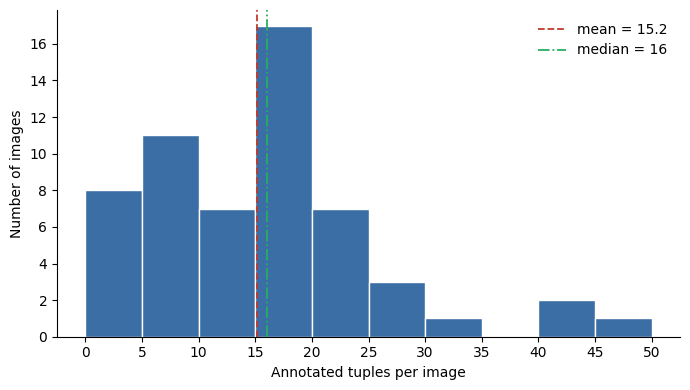
\includegraphics[width=0.8\linewidth]{tuples_per_image_hist.png}%
  }{%
    \fbox{\parbox[c][0.34\textheight][c]{0.8\linewidth}{\centering\itshape
      Tuples-per-image histogram --- placeholder. Replace with the provided
      plot \texttt{tuples\_per\_image\_hist.png} (number of tuples per image
      across the 57-image corpus).}}%
  }
  \caption[Tuples per image]{%
    Number of tuples per image, across the $57$ images. The mean is $15.2$
    and the median is $16$. Most images are small; a few dense tables form a
    long tail.}
  \label{fig:tuples-per-image}
\end{figure}

The images split into three groups by tuple count: \emph{sparse}
($1$--$9$), \emph{medium} ($10$--$20$), and \emph{dense} ($21$ or more).
Table~\ref{tab:density-bands} gives the split. Most images are medium
($50.9\%$ of images, $54.5\%$ of tuples). The outer groups are uneven:
sparse images are a third of the images ($33.3\%$) but only $12.2\%$ of the
tuples, and dense images are the opposite ($15.8\%$ of images, $33.3\%$ of
tuples).

\begin{table}[tb]
  \centering
  \caption[Image-density bands]{%
    Images grouped by tuple count. Dense images are $15.8\%$ of the images
    but hold a third of the tuples.}
  \label{tab:density-bands}
  \begin{tabular}{lrrrr}
    \toprule
    Band              & Images & \% Images & Tuples & \% Tuples \\
    \midrule
    Sparse (1--9)     & 19 & 33.3  & 106 & 12.2  \\
    Medium (10--20)   & 29 & 50.9  & 472 & 54.5  \\
    Dense ($\geq 21$) &  9 & 15.8  & 288 & 33.3  \\
    \midrule
    Total             & 57 & 100.0 & 866 & 100.0 \\
    \bottomrule
  \end{tabular}
\end{table}

This matters for scoring. The metric counts every tuple equally across the
corpus, so images with more tuples affect the score more, and the dense
images carry most of the weight. They are also the hardest, with many
nutrients, repeated columns, and sometimes poor OCR. One, \texttt{15.PNG},
has the only three-column layout in the corpus and a large OCR failure; it
returns later and in Chapter~\ref{chap:experiments}.

\FloatBarrier

\section{Annotation Schema and Protocol}\label{sec:schema}

This section defines a tuple and explains how the tuples were made: first
the schema, then the two-pass annotation, then the step that normalises the
nutrient names.

\subsection{The annotation schema}\label{sec:schema-tuple}

Each tuple is a row of seven fields, listed with an example in
Table~\ref{tab:schema}. One field, \texttt{image\_id}, names the source
image. Four fields are the extraction target and the tuple scored by the
metric (the four-field target of Chapter~\ref{chap:methodology}):
\texttt{nutrient} is the nutrient name, \texttt{quantity} is a number,
\texttt{unit} is the unit, and \texttt{context} is the basis the value is
given under (\texttt{per\_100g}, \texttt{per\_serving},
\texttt{per\_daily\_dose}, or \texttt{per\_100ml}).

Two fields are auxiliary. \texttt{nrv\_percent} is the reference-value
percentage, as a plain number. \texttt{serving\_size} is the serving or
dose, as free text; when a tuple has one, it is added to the
\texttt{context} value before scoring (for example,
\texttt{per\_serving (Pro Stick)}). Both fields are often empty, for reasons
given later in this chapter.

\begin{table}[tb]
  \centering
  \caption[The annotation schema]{%
    The seven fields, with an example row from image \texttt{106.PNG}. The
    four middle fields are the scored tuple. \texttt{serving\_size}, when
    present, is added to \texttt{context} before scoring.}
  \label{tab:schema}
  \begin{tabular}{lll}
    \toprule
    Field & Content & Example \\
    \midrule
    \texttt{image\_id}     & source image                    & \texttt{106.PNG}      \\
    \texttt{nutrient}      & nutrient name                   & Magnesium             \\
    \texttt{quantity}      & number only                     & 250                   \\
    \texttt{unit}          & unit                            & mg                    \\
    \texttt{context}       & reference basis                 & \texttt{per\_serving} \\
    \addlinespace
    \texttt{nrv\_percent}  & reference-value \%, number only & 67                    \\
    \texttt{serving\_size} & serving / dose, free text       & Pro Stick             \\
    \bottomrule
  \end{tabular}
\end{table}

Two points about the schema matter later. First, the quantity and the unit
are separate fields, and the quantity is only a number, so the unit can
change without changing the value. Second, nutrient names are kept in the
language printed on the label; they are mapped to one common form in a later
step (\S\ref{sec:schema-normalisation}), which changes only the nutrient
field.

\subsection{Two-cycle annotation}\label{sec:schema-annotation}

The tuples were made in two passes. In the first pass, a large
vision--language model (Gemini~3) read each image and wrote out its tuples
in the schema above. It was told to copy only visible text, invent nothing,
and keep nutrient names in their original language. Each quantity was a
number with the unit in a separate field. Context headers were mapped to
the fixed forms, breakdown entries such as single magnesium salts became
separate rows, qualifiers such as ``(gesamt)'' were kept, the percent sign
was dropped from the NRV field, and a field was left empty when the label
gave no value. Rows were not merged, so an energy line in both kJ and kcal
became two rows.

The second pass was manual. The author checked the model's output against
each image, corrected misreadings, added missing rows, and removed wrong
ones. This checked output is the gold standard; the first pass only saved
manual typing.

One of the baselines in Chapter~\ref{chap:experiments} is also a
vision--language model, so three facts are worth noting. The labels are
defined by the human pass, not the model: every row was checked by hand.
The model used for annotation (Gemini~3) is not the baseline model (the
smaller Gemma~3~4B). And the pipeline does not use the annotations at all.

\subsection{Nutrient-name normalisation}\label{sec:schema-normalisation}

The labels print the same nutrient in many forms: \texttt{Eiwei{\ss}},
\texttt{EIWEISS}, and \texttt{Protein} all mean protein. A final step maps
these to one common name, so a predicted name and a gold name can be
compared as strings. It changes only the nutrient field.

The mapping has three tiers. A name is first looked up in a dictionary of
exact forms. If it is not found, it is split on the separators labels use
for two languages (``Fett\,/\,fat''), and the first part is matched against
a set of patterns. A name that matches neither is kept as it is.

This has two effects, both used in the next section. First, common
nutrients become one English name (\texttt{Eiwei{\ss}} to \texttt{Protein},
``davon Zucker'' to \texttt{Sugars}), while rare names that appear once or
twice --- specific magnesium salts, plant extracts, probiotic strains ---
keep their German or Latin form. So the names are mixed: English for common
nutrients, German or Latin for rare ones. Second, the step flattens the
``of which'' rows, so a sub-nutrient such as ``davon Zucker'' is stored as
its own nutrient (\texttt{Sugars}) rather than under the one above it. After
this step the corpus has $62$ different nutrient names.

Two final points. The dictionary keeps some names apart even when they mean
the same thing: \texttt{Colecalciferol} and \texttt{Vitamin~D3} stay
separate and are counted as two. And the pipeline applies the same mapping
to its own output (rule~C15 in Chapter~\ref{chap:methodology}), so gold and
predicted names use the same vocabulary when compared.

\FloatBarrier

\section{The Four Fields}\label{sec:fields}

This section looks at the four scored fields one by one: nutrient,
quantity, unit, and context. Each has a pattern that makes it hard to read
off the label, and the context field explains why the pipeline builds a
graph.

\subsection{Nutrient names}\label{sec:fields-nutrient}

The corpus has $62$ different nutrient names, used very unevenly. The top
five cover $447$ tuples ($51.6\%$), the top ten cover $644$ ($74.4\%$), and
the top fifteen cover $713$ ($82.3\%$). Figure~\ref{fig:nutrient-top15}
shows the fifteen most common. Fifteen names ($24.2\%$ of the vocabulary)
appear only once.

\texttt{Energy} is the most common, at $152$ tuples, about twice the next.
This is because most labels print energy in both kilojoules and
kilocalories, and each is a separate tuple; counted as one nutrient, energy
would be about $76$, like fat, carbohydrate, and protein.

\begin{figure}[tb]
  \centering
  \IfFileExists{nutrient_top15.png}{%
    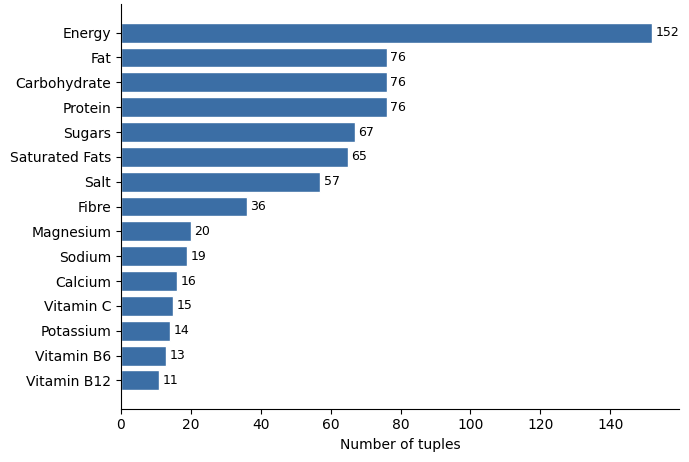
\includegraphics[width=0.85\linewidth]{nutrient_top15.png}%
  }{%
    \fbox{\parbox[c][0.34\textheight][c]{0.85\linewidth}{\centering\itshape
      Top-nutrient figure --- placeholder. Replace with the provided plot
      \texttt{nutrient\_top15.png} (the fifteen most common nutrient names by
      tuple count).}}%
  }
  \caption[Most common nutrient names]{%
    The fifteen most common nutrient names, by tuple count. \texttt{Energy}
    is highest because most labels state it twice, in kJ and kcal. The corpus
    has $62$ names in total, $15$ of which appear only once.}
  \label{fig:nutrient-top15}
\end{figure}

\subsection{Quantities}\label{sec:fields-quantity}

Almost all quantities are plain numbers: of the $866$ values, $846$ are
plain numbers, $18$ are bounds such as \texttt{<0.1}, and $2$ are in
scientific notation (Table~\ref{tab:quantity-formats}). The bounds are trace
amounts, mostly for salt or sodium. The two scientific-notation values are
bacteria counts ($3.6\times10^{8}$) on two probiotic rows.

The values cover a very wide range. The plain values run from $0.02$ to
$10\,000$, about $5.7$ orders of magnitude; with the two bacteria counts,
the range grows to about $10$ orders of magnitude. About one value in ten is
zero ($86$ of $866$), from labels stating zero sugar, fat, or salt, and none
are negative.

\begin{table}[tb]
  \centering
  \caption[Quantity formats]{%
    The three quantity formats. Almost all values are plain numbers; the
    rest are trace bounds or bacteria counts.}
  \label{tab:quantity-formats}
  \begin{tabular}{lrl}
    \toprule
    Format               & Count & Example \\
    \midrule
    Plain number         & 846 & $250$              \\
    Bound                & 18  & \texttt{<0.1}      \\
    Scientific notation  & 2   & $3.6\times10^{8}$  \\
    \bottomrule
  \end{tabular}
\end{table}

\subsection{Units}\label{sec:fields-unit}

The corpus uses $11$ units, but five cover almost everything: grams,
milligrams, micrograms, kilocalories, and kilojoules together cover $97.5\%$
of the tuples, and grams alone cover $55.5\%$
(Figure~\ref{fig:unit-distribution}). The other six are rare and fall into
two kinds. The first is equivalence units, written as a mass unit plus a
suffix, one per vitamin: mg~$\alpha$-TE for vitamin E, mg~NE for niacin,
µg~RE for vitamin A. The second is activity and count units: I.E. for
vitamin D and KBE for the probiotic strains.

\begin{figure}[tb]
  \centering
  \IfFileExists{unit_distribution.png}{%
    
\includegraphics[width=0.85\linewidth]{unit_distribution.png}%
  }{%
    \fbox{\parbox[c][0.34\textheight][c]{0.85\linewidth}{\centering\itshape
      Unit-distribution figure --- placeholder. Replace with the provided
      plot \texttt{unit\_distribution.png} (the 11 units by tuple count).}}%
  }
  \caption[Unit distribution]{%
    The $11$ units, by tuple count. Five units (g, mg, µg, kcal, kJ) cover
    $97.5\%$ of the tuples. The rest are equivalence units (such as
    mg~$\alpha$-TE) and count units (I.E., KBE).}
  \label{fig:unit-distribution}
\end{figure}

\subsection{Contexts}\label{sec:fields-context}

There are four context values: \texttt{per\_100g} ($44.0\%$),
\texttt{per\_serving} ($37.3\%$), \texttt{per\_daily\_dose} ($15.0\%$), and
\texttt{per\_100ml} ($3.7\%$). They split into two kinds. \texttt{per\_100g}
and \texttt{per\_100ml} are reference amounts; a label uses one or the
other, never both. \texttt{per\_serving} and \texttt{per\_daily\_dose} are
portions. A label can combine one reference amount with one or more
portions.

Most labels use more than one context. Of the $57$ images, $37$ ($64.9\%$)
have two or more contexts, and by tuples the share is higher: $707$ of $866$
($81.6\%$) come from these images. The most common layout is
\texttt{per\_100g} with \texttt{per\_serving}, in $27$ images
(Figure~\ref{fig:context-structure}).

This is why the pipeline needs more than a left-to-right reading. In a
multi-context label, one nutrient name has several values, one per column.
Across the corpus, $313$ of $463$ nutrient instances ($67.6\%$) have two or
more values, one per context. The name appears once but must link to two or
three different values, and the only thing separating them is which column
they sit in. A line-by-line reader cannot tell them apart; it has to use the
column positions, which is what the graph in Chapter~\ref{chap:methodology}
encodes. \texttt{15.PNG} is the hardest case, with three contexts at once,
so each nutrient links to three values.

\begin{figure}[tb]
  \centering
  \IfFileExists{context_structure.png}{%
    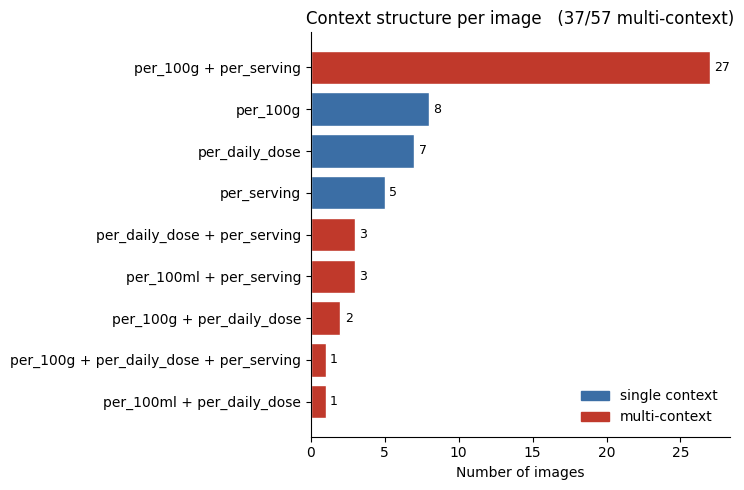
\includegraphics[width=0.85\linewidth]{context_structure.png}%
  }{%
    \fbox{\parbox[c][0.34\textheight][c]{0.85\linewidth}{\centering\itshape
      Context-layout figure --- placeholder. Replace with the provided plot
      \texttt{context\_structure.png} (context layouts across the 57
      images).}}%
  }
  \caption[Context layouts]{%
    Context layouts across the $57$ images. $37$ images ($64.9\%$) use more
    than one context. The most common layout is \texttt{per\_100g} with
    \texttt{per\_serving}.}
  \label{fig:context-structure}
\end{figure}

\FloatBarrier

 
\section{Field Completeness}\label{sec:completeness}
 
The four scored fields are almost always present. Nutrient, quantity, and
context are filled in every tuple; unit is missing in only one (an energy
value printed with no unit). So $865$ of $866$ tuples ($99.9\%$) have all
four scored fields, and the four-field tuple is well-posed for almost every
row. Figure~\ref{fig:completeness} shows the rates.
 
The two extra fields are often empty: \texttt{nrv\_percent} is filled in
$20.2\%$ of tuples and \texttt{serving\_size} in $57.6\%$. Both gaps are
structural, not missing work. \texttt{nrv\_percent} is mostly a
micronutrient field: vitamins and minerals carry a reference-value
percentage, while most macronutrient rows do not print one, so the field is
blank there because the label has no value. \texttt{serving\_size} follows
the context. It is almost always present on portion contexts
(\texttt{per\_serving}, \texttt{per\_daily\_dose}) and almost never on
reference contexts (\texttt{per\_100g}, \texttt{per\_100ml}), because a
serving size only makes sense for a portion. It is a property of the panel,
not of each row, and when present it is folded into the context value, as
\S\ref{sec:schema-tuple} describes.
 
\begin{figure}[tb]
  \centering
  \IfFileExists{field_completeness.png}{%
    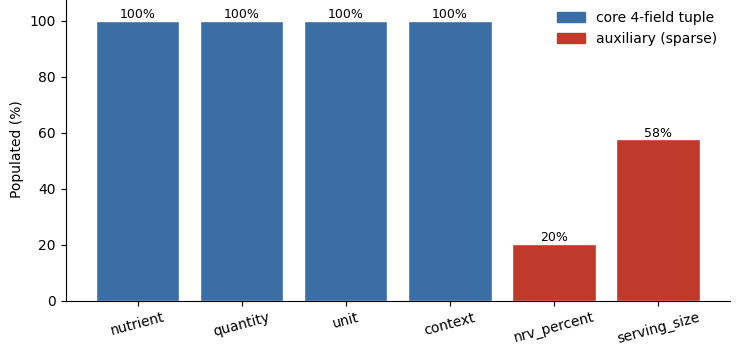
\includegraphics[width=0.8\linewidth]{field_completeness.png}%
  }{%
    \fbox{\parbox[c][0.34\textheight][c]{0.8\linewidth}{\centering\itshape
      Field-completeness figure --- placeholder. Replace with the provided
      plot \texttt{field\_completeness.png} (share of tuples with each field
      filled).}}%
  }
  \caption[Field completeness]{%
    Share of tuples with each field filled. The four scored fields are
    near-complete; \texttt{nrv\_percent} and \texttt{serving\_size} are
    sparse for structural reasons.}
  \label{fig:completeness}
\end{figure}
 
\FloatBarrier
  

% =====================================================================
%  Insert immediately BEFORE  \section{Evaluation}\label{sec:evaluation}
%  (after the \FloatBarrier that closes "Field Completeness").
%  booktabs + graphicx only (already loaded). No new figure asset.
% =====================================================================

\section{The Reduced Test Set}\label{sec:testset}

All of the labels described so far belong to the corpus, and the experiments in
Chapter~\ref{chap:experiments} are run across it. Two of them, however, are not
tables. They lack the row-and-column layout the method needs in order to pair a
nutrient with its values, which places them outside what the pipeline is built
to read. Because both were part of that data, their effect is shown directly:
the runs are scored a second time with the two labels removed, and the figures
for the full corpus and for the reduced set appear side by side.

The two labels are \texttt{15.PNG} and \texttt{67.jpeg}. Between them they hold
$46$ tuples, and the split is very uneven: $42$ come from \texttt{15.PNG}, one of
the largest labels in the whole corpus, and only $4$ from \texttt{67.jpeg}.
Taking both out leaves $55$ images and $820$ tuples, so nearly all of the
reduction traces to one dense label rather than to the pair together.

In shape, the reduced set differs only slightly from the full one.
Table~\ref{tab:testset} sets the two beside each other. The typical image is
unchanged in size: the median holds at $16$ tuples, and the mean falls just a
little, from $15.2$ to $14.9$. Contexts and units keep almost the same balance
as before, and the vocabulary loses a single name, from $62$ down to $61$,
because \texttt{Colecalciferol} was printed on a removed label and nowhere else.
Across the four scored fields the reduced set stays near-complete, with every one
of the $820$ tuples carrying a nutrient, a quantity and a context, and only one
missing its unit.

\begin{table}[tb]
  \centering
  \caption[Full corpus versus reduced test set]{%
    The full corpus and the reduced set, the latter with the two non-tabular
    labels removed. Chapter~\ref{chap:experiments} reports scores on both.
    Percentages are shares of tuples within each set.}
  \label{tab:testset}
  \begin{tabular}{lrr}
    \toprule
                              & Full corpus & Reduced set \\
    \midrule
    Images                    & 57   & 55   \\
    Tuples                    & 866  & 820  \\
    Distinct nutrients        & 62   & 61   \\
    Tuples per image (mean)   & 15.2 & 14.9 \\
    Tuples per image (median) & 16   & 16   \\
    \addlinespace
    \texttt{nutrient} filled  & 866  & 820  \\
    \texttt{quantity} filled  & 866  & 820  \\
    \texttt{unit} filled      & 865  & 819  \\
    \texttt{context} filled   & 866  & 820  \\
    \addlinespace
    \texttt{per\_100g}        & 44.0\% & 44.8\% \\
    \texttt{per\_serving}     & 37.3\% & 37.4\% \\
    \texttt{per\_daily\_dose} & 15.0\% & 13.9\% \\
    \texttt{per\_100ml}       & 3.7\%  & 3.9\%  \\
    \bottomrule
  \end{tabular}
\end{table}

One difference deserves a note, as it links back to the earlier account of
context. Of all the annotated labels, \texttt{15.PNG} alone recorded three
contexts at once. With it gone, nothing in the reduced set holds more than two,
so a nutrient name maps to two values at most rather than three. None of this
weakens the case for a graph. About two nutrient instances in three ($298$ of
$448$, or $66.5\%$) still fall under more than one context, and what separates
those values is only the column they occupy. That one label had simply shown the
pattern in its most extreme form.

\FloatBarrier



\section{Evaluation}\label{sec:evaluation}
 
The pipeline is scored by comparing its output tuples against the gold
tuples. This section defines when a tuple counts as correct, and how
predicted tuples are matched to gold tuples to compute the score.
 
\subsection{What counts as a correct tuple}\label{sec:metric}
 
A predicted tuple is correct when it matches a gold tuple in all four
fields. Each field is compared up to normalisation, so that surface
differences do not count as errors:
\begin{itemize}
  \item the \texttt{nutrient} is matched by name, allowing for differences in
        case and in German or English spelling;
  \item the \texttt{quantity} is matched by its numeric value;
  \item the \texttt{unit} is matched after treating equivalent unit names as
        the same (for example µg and mcg), while keeping kJ and kcal
        distinct;
  \item the \texttt{context} is matched as its canonical basis
        (\texttt{per\_100g}, \texttt{per\_serving}, \texttt{per\_daily\_dose},
        \texttt{per\_100ml}).
\end{itemize}
 
A tuple that matches on all four fields is a four-field (4F) match. A tuple
that matches on nutrient, quantity, and unit, ignoring context, is a
three-field (3F) match. The 4F match is the primary metric of this work; the
3F match is reported alongside it to show how much the context field costs.
 
\subsection{Matching predictions to gold}\label{sec:protocol}
 
The evaluator is deterministic: it applies the fixed rules above in a single
pass, with no model in the loop. It works per image, and the counts are then
pooled over the corpus.
 
For each image, the predicted tuples are matched to the gold tuples one to
one. Matching is greedy: the predicted tuple whose nutrient name is closest
to a gold name is paired first, with quantity and unit breaking ties, and
each gold tuple and each predicted tuple is used at most once. Each matched
pair is then scored field by field. A gold tuple with no matching prediction
is a miss, and a predicted tuple with no matching gold is a false alarm.
 
\subsection{Field-level and tuple-level scores}\label{sec:scores}
 
The pipeline is scored at two levels.
 
\paragraph{Field level.} Each field is checked on its own, over the matched
pairs. The quantity accuracy is the share of matched tuples with the right
quantity; unit and context accuracy are the same. These rates show which
field is the weak point, but they only cover tuples that were matched in the
first place.
 
\paragraph{Tuple level.} The whole tuple is judged together and counts as
correct only if all four fields match (or three, for 3F). This is the
strict, headline measure, and it uses three numbers:
\begin{itemize}
  \item \emph{precision} is the share of predicted tuples that are correct;
        it drops when the pipeline outputs wrong or extra tuples;
  \item \emph{recall} is the share of gold tuples that are found; it drops
        when the pipeline misses tuples;
  \item \emph{F1} is the harmonic mean of precision and recall --- one number
        that is high only when both are high.
\end{itemize}
The tuple-level scores are pooled over all $866$ gold tuples, so every tuple
counts equally (\S\ref{sec:corpus}). The 4F F1 is the primary metric of this
work, with 3F F1 reported alongside.
 
\FloatBarrier